\chapter{Software development process}
\label{chapter:Analysis tool}

\begin{introduction}
    “I've learned a painful lesson, that for small programs dynamic typing is great. For large programs, you have to have a more disciplined approach. And it helps if the language actually gives you that discipline, rather than telling you, 'Well, you can do whatever you want.'” - Guido van Rossum, Python's creator
\end{introduction}

Falar de Metodologia Agile

\section{Requirements}

This section presents the requirements for the developed software, categorized into functional and non-functional requirements. 
\subsection{Functional Requirements}

Functional requirements specify the functionalities that end-users require as essential components of the system. They describe the system's behavior in terms of inputs, operations to be performed, and expected outcomes. These requirements are directly observable by users in the final product. \cite{Geeks2024} The main functional requirements of the developed software are:

\subsubsection{\textbf{FR1 - Collection of BAM/CRAM Files for Analysis}}

The software must enable the collection of BAM/CRAM sequencing files stored on the company's servers.

\subsubsection{\textbf{FR2 - Calculation of Depth of Coverage/Read Depth and Coverage/Breadth of Coverage}}

The software must facilitate the calculation of Depth of Coverage and Coverage/Breadth of Coverage for the collected BAM/CRAM files. Users should be able to configure analysis parameters, such as selecting regions of interest within the exome. The analysis should be based on a universal BED file containing exon coordinates. The analysis should use bioinformatics tools like SAMtools, which returns a .depth file with results that must be processed by the software to obtain the desired metrics.

\subsubsection{\textbf{FR3 - Graphical User Interface}}

The software must have a graphical user interface that allows users to interact with the system in an intuitive and efficient manner. The interface should be simple and easy to use, enabling users to collect BAM/CRAM files, configure analysis parameters, and view the obtained results. The interface should be developed using Streamlit, a Python web development tool that allows the creation of interactive web applications with minimal code. It should support user interaction through widgets such as buttons, text boxes, sliders, and others. The interface should allow filtering of results and exporting results to a CSV file.

\subsection{Non-Functional Requirements}

Non-functional requirements refer to the quality attributes of the software, such as performance, usability, security, and scalability. These requirements are crucial to ensure that the software operates efficiently, is secure, and can be easily used by various user profiles. \cite{Geeks2024} The main non-functional requirements of the system are described as follows:

\subsubsection{\textbf{NFR1 - Usability}}

The software should be intuitive and user-friendly, enabling even users with no technical background to interact with the system efficiently. The graphical user interface should be simple and clear, with straightforward instructions on how to use the system. It should allow users to collect BAM/CRAM files, configure analysis parameters, and view results quickly and easily. Clear and informative error messages should be provided in case of task execution failures, along with instructions for resolving issues.

\subsubsection{\textbf{NFR2 - Performance}}

The software must be optimized to process large volumes of sequencing data, ensuring that the calculation of Depth of Coverage/Read Depth and Coverage/Breadth of Coverage occurs within a reasonable time frame. The possibility of parallelizing calculations should be explored, utilizing multicore or distributed resources to accelerate data processing.

\subsubsection{\textbf{NFR3 - Scalability}}

The system must be scalable, capable of handling significant increases in data volume or the number of users without compromising performance. This includes the ability to leverage cloud services such as AWS S3. The software should be designed to allow the addition of new modules or functionalities without the need to rewrite the core code, ensuring flexibility for future evolution of the system.

\subsubsection{\textbf{NFR4 - Security and Data Privacy}}

The software must protect sensitive data, especially patient-related data, in compliance with regulations such as General Data Protection Regulation (GDPR). Temporary data used during processing must be properly deleted after analysis, ensuring data privacy and security. System access should be controlled through authentication and authorization, ensuring that only authorized users can interact with the system. A logging system should be implemented to record user activities and monitor system usage.

\subsubsection{\textbf{NFR5 - Portability and Compatibility}}

The software should be implemented on Windows but must ensure access to a Linux environment using WSL. It should guarantee easy integration with tools like Samtools in the WSL environment without requiring advanced configuration by the end user.

\subsubsection{\textbf{NFR6 - Maintainability}}

The software code must be modular and well-documented, facilitating easy maintenance and extension of the system in the future. Best development practices, such as version control (Git), should be applied, ensuring that the code can be managed efficiently over time. Software updates should be simple to implement, and developer documentation should include clear instructions on how to add new functionalities or adjust existing behaviors.

With clear definitions of functional and non-functional requirements, the development of the software was structured efficiently, ensuring it meets both technical expectations and operational needs of the company and end-users. Considering these requirements throughout the development cycle was crucial for the success of the project.



\section{System Design and Architecture}

The developed software is based on a web interface accessible through a browser, using the Streamlit library to build the application. The interface is composed of several interactive widgets that allow the user to configure and execute different types of genomic analysis: Single Gene, Gene Panel, or Exome.

\subsection{User Workflow}

Initially, the user must select the type of analysis they wish to perform. Depending on the selection, the processing flow adapts to optimize both the user experience and the efficiency of the necessary calculations.

\subsubsection{\textbf{Single Gene Analysis}}

The user uploads a BAM or CRAM file, containing the sequencing data. Additionally, they automatically receive a universal BED file corresponding to the selected genome assembly. The user then chooses the gene of interest and may specify the exon(s) to be analyzed. SAMTOOLS is invoked to generate a DEPTH file, which contains information about the read depth at each genomic position. This file is processed by a Python script that calculates two key metrics: depth of coverage and breadth of coverage. The results are displayed to the user through a report in the Streamlit interface or can be exported as a CSV file.

\subsubsection{\textbf{Gene Panel Analysis}}

Similar to the Single Gene analysis, the user uploads a BAM/CRAM file and receives the universal BED file. However, in this case, the user selects the gene panel for the analysis instead of a single gene. The corresponding BED file is processed by SAMTOOLS to generate the DEPTH file, which is then used to calculate the same coverage metrics. The result visualization and export process follow the same steps as in the Single Gene analysis.


\subsubsection{\textbf{Exome Analysis}}

In Exome analysis, the entire exome is used for the analysis, without requiring the selection of a specific region. The user uploads the BAM/CRAM file, and the universal BED file corresponding to the exome is utilized. As in the other modes, SAMTOOLS generates the DEPTH file, which is processed to calculate the coverage metrics. The results are displayed or exported in the same manner.


The modular design of the software allows for seamless integration between various components, namely Streamlit for the interface, SAMTOOLS for processing sequencing data, and Python scripts for calculating coverage metrics. Each of these steps is interconnected to provide the user with quick, accurate, and real-time results. The software's architecture is designed to be easily scalable and adaptable to different types of genomic analysis, supporting both focused and large-scale analyses (such as whole exome).

The Figure \ref{fig:architecture} shows the scheme of the software architecture, highlighting the main components.
\begin{figure}[H]
    \centering
    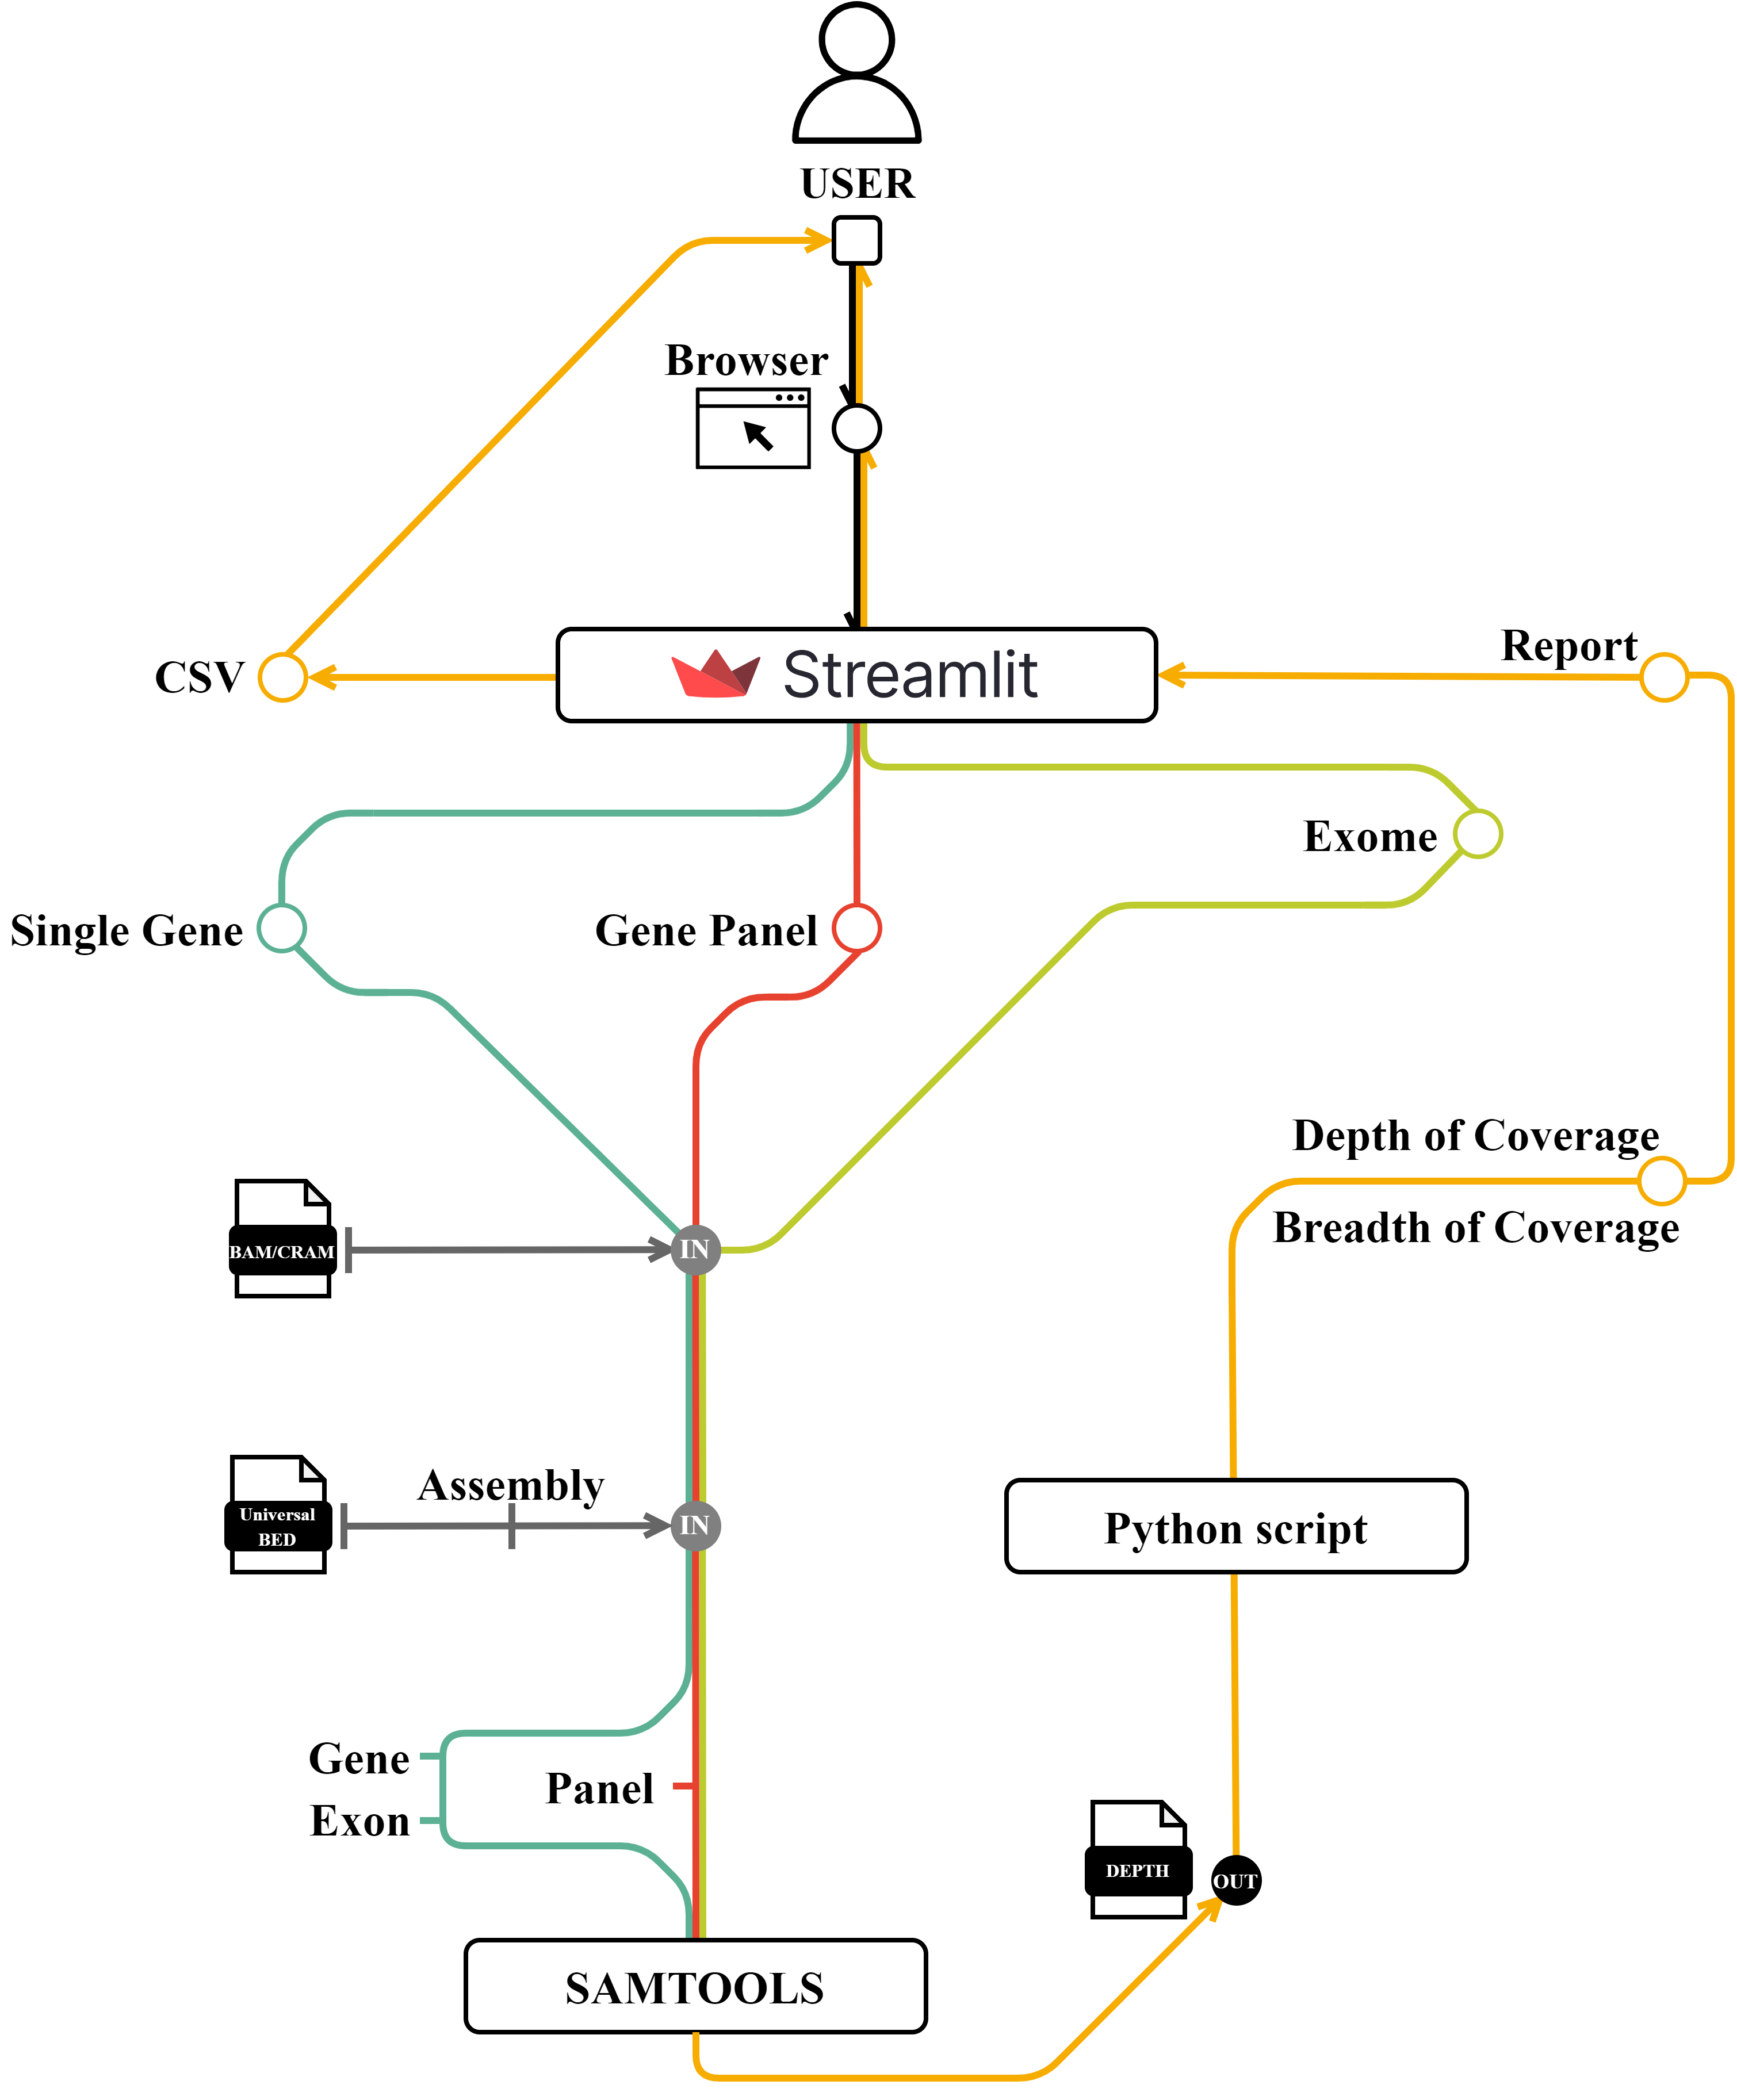
\includegraphics[width=0.7\textwidth]{figs/architecture.png}
    \caption{Scheme of the software architecture.} 
    \label{fig:architecture}
\end{figure}


The project is organized in a modular structure to support the development of a metrics-based application. At the top level, the \texttt{metrics\_app} directory contains core components such as the app logic and necessary resources. The \texttt{app} folder houses the main scripts that drive the application, including \texttt{Home.py}, which serves as the entry point, and submodules like \texttt{app\_pages} for UI-specific components such as \texttt{about.py}, \texttt{query.py}, and \texttt{results.py}. The \texttt{components} directory contains functional modules such as \texttt{analysis.py}, \texttt{metrics.py}, and \texttt{bam\_cram.py}, encapsulating core logic for genome analysis, metrics computation, and file handling. The \texttt{data} folder stores essential files, including genomic depth and region data, which are organized by specific analysis types (e.g., exome, gene panel). The project includes setup files like \texttt{environment.yml} for managing dependencies and a \texttt{Dockerfile} to enable containerization for consistent deployment. Overall, the structure supports scalability, modularity, and ease of maintenance. The Figure \ref{fig:tree} shows the software directory structure.

\begin{figure}[H]
    \centering
    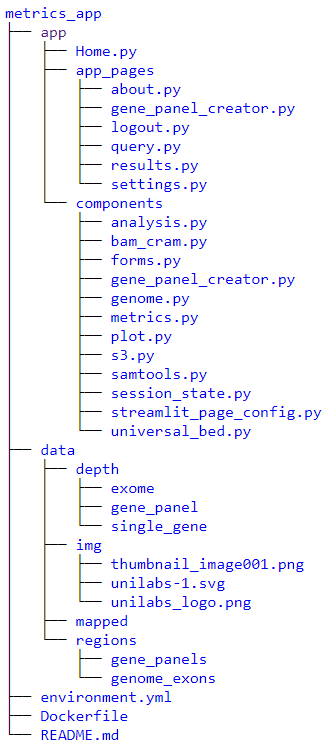
\includegraphics[width=0.3\textwidth]{figs/tree.png}
    \caption{Software directory structure.} 
    \label{fig:tree}
\end{figure}


\section{Development}

The development of the software followed an iterative and structured approach, with each stage focusing on expanding its functionality while ensuring stability and performance. The process began with the implementation of the Single Gene analysis, which served as the foundation for the project. This initial version was designed to be stable and functional, enabling users to upload BAM or CRAM files and analyze specific genes and exons with precision.

Once the Single Gene functionality was fully operational, the next phase involved adding support for Gene Panel analysis. This required adjusting the existing framework to handle a broader set of genes while maintaining the same level of accuracy and efficiency. A stable and functional version was again achieved, providing users with the ability to select and analyze predefined gene panels.

Finally, the software was further enhanced to include Exome analysis, allowing for the comprehensive examination of the entire exome. This functionality was integrated without compromising the stability or performance of the system, and once again, a stable and functional version was built.

Throughout the development, various components and tools were employed to ensure the software met the required performance standards and provided an intuitive user experience. The careful progression from Single Gene to Gene Panel, and finally to Exome analysis, highlights the modularity and scalability of the software, as well as the emphasis placed on testing and validation at each stage.

The following sections provide an overview of the key tools and technologies used in the development of the whole software, including all the stages of the project.
\subsection{Environment preparation }
\subsubsection{\textbf{Windows Subsystem for Linux (WSL)}}

On Windows, developers have access to both the Windows and Linux environments, thanks to the Windows Subsystem for Linux (WSL). With WSL, it is possible to install different Linux distributions, such as Ubuntu, OpenSUSE, Kali, Debian, Arch Linux, among others. This allows Linux applications, utilities and command-line tools to be used directly in Windows, without the need to modify the operating system, resort to virtual machines or dual boot. \cite{wsl}

In the context of the development of this tool, the need to install WSL was driven mainly due to the scenario in which many essential tools and software for bioinformatics are designed to work in Linux environments. For this reason, we followed the set of steps recommended on the Microsoft website to configure this environment (Build 19041 or higher). \cite{wsl}

\subsubsection{\textbf{Anaconda and Conda}}

After installing WSL, the installation step of Anaconda followed, a platform for data science in Python/R that includes conda, a package and environment manager, making it easier for users to manage a collection of more than 7,500 open source packages. \cite{anaconda1}

In the case of the creation of the metrics analysis tool, this step was fundamental to allow the installation and maintenance of all the packages and dependencies necessary for the operation of the software. By creating a conda environment, it was possible to ensure that all installed tools work independently without conflicts between versions and packages, thus ensuring the reproducibility of the created software. \cite{anaconda2}

Following the documentation provided by Anaconda, the installation and creation of the conda environment was carried out. \cite{anaconda3} 

Additionally, all the dependencies of the Table \ref{tab:packages} were installed within the created environment. This installation was carried out by installing package by package, however, an environment.yaml file was made available that allows the bulk installation \cite{anaconda4} of all dependencies on the versions compatible with the software.

\subsubsection{\textbf{Git and GitHub}}

GitHub is a platform that allows users to store, share, and collaborate on code writing with others. \cite{github}

Its operation is based on repositories managed by Git, a version control system that tracks all changes made by one or more users in a project. \cite{github}

When files are uploaded to GitHub, they become part of the created repository. Any change (commit) to any file is automatically tracked. These changes, made locally, are usually synchronized continuously by pushing the committed changes. Similarly, any changes made locally by another user and synchronized on GitHub can be retrieved by making a pull request. \cite{github}

Thus, by using the documentation of Git and GitHub, this practice was implemented, which not only ensures that each version of the created software is recorded—guaranteeing that the work is not lost and allowing for version rollback in case of bugs—but also ensures that all software produced is reproducible and available for deployment by any user. \cite{github}

\subsection{Streamlit}

The developed software was built using Streamlit which is an open-source Python library designed to enable the swift and intuitive creation of interactive web applications, primarily aimed at data science and machine learning projects. Introduced in October 2019 and now part of the Snowflake ecosystem, Streamlit has quickly gained recognition within the data science community due to its user-friendly approach. Its main goal is to make transforming machine learning scripts into interactive apps as simple as possible, allowing users to incorporate complex features with minimal effort. \cite{Sehm2022}

Streamlit's core philosophy revolves around a declarative, straightforward interface-building model. It enables developers to create apps using clean, concise code without the need for managing intricate state or setting up callbacks, which is common in other frameworks. This makes Streamlit especially suited for rapid prototyping, as well as for displaying machine learning models and data visualizations. The library also seamlessly integrates with many popular Python frameworks for data analysis and visualization. \cite{Sehm2022}

What further sets Streamlit apart is its flexibility and extensibility. The library's architecture allows the integration of various web components, making it easy to customize applications for different use cases. This versatility, along with its growing popularity and adoption in the data science world, has cemented Streamlit as a valuable tool for building interactive, informative applications that can be easily shared and adapted. \cite{Dayanithi2023}

Various Streamlit widgets were used to create the graphical interface of the software, including buttons, text boxes, selectors, among others. Additionally, the library was employed to display the analysis results, also allowing data export to a CSV file. The integration of Streamlit with Python was crucial in developing an interactive and user-friendly software, meeting the established usability requirements. The functionality and implementation of these widgets are detailed in \cite{streamlit_doc}.

\subsection{Processing and Simplification of BED File for Genomic Analysis}

The original BED files utilized in this study, \textbf{hg19\_Twist\_ILMN\_Exome\_2.0\_Plus\_Panel\_annotated.bed} for GRCh38/hg38 assembly and \textbf{hg38\_Twist\_ILMN\_Exome\_2.0\_Plus\_Panel\_annotated.bed} for GRCh37/hg19 assembly, was highly complex due to its rich annotation, particularly in the fourth column, which contained multiple genes and clinical identifiers associated with the same genomic region. For instance, a single entry could include a large number of comma-separated values representing multiple genes and clinical IDs. Such complexity was unnecessary for our specific analysis, which focused primarily on gene panel-level, gene-level and exon-level metrics. Therefore, it was essential to simplify the file while preserving relevant genomic data, particularly the coodinates, gene names and exon numbers.

The simplification process involved writing a custom Python script designed to extract and reorganize key elements from the original BED file. The script processes each line of the file, extracting the chromosome, start, and end positions, while simplifying the fourth column to retain only the first gene listed. Additionally, the script calculates exon numbers for each gene based on the sequence of occurrences in the file. This transformation results in a more concise representation, which is more suitable for downstream analysis.

The original file included regions defined by start and end positions of genomic intervals, as well as various annotations. A key challenge was to disambiguate the fourth column, where multiple genes and identifiers were grouped together. The Python script divided the contents of this column by the comma delimiter and selected only the first gene. In doing so, it reduced complexity while retaining a representative gene for each genomic region.

Another critical aspect of the transformation was the counting of exons for each gene. The script tracks changes in the gene name between consecutive lines and increments an exon count whenever a new gene is encountered. This ensures that each gene is assigned a unique exon number, allowing for consistent tracking of exon-level metrics. Additionally, the script calculates the length of each genomic interval by subtracting the start position from the end position.

To facilitate downstream analysis and ensure compatibility with different tools, the script also included an option to remove the "chr" prefix from chromosome identifiers. This was particularly important for certain bioinformatics tools that require the chromosome numbers without this prefix. The option to remove the prefix was controlled by a boolean flag, ensuring flexibility in handling different file formats.

The output of this process was a simplified BED file containing six columns: chromosome number, start position, end position, gene name, exon number, and exon length (calculated as the difference between the start and end positions). Below is an example of the resulting file structure:

\begin{verbatim}
    
    (...)
    17	41177976	41178064	RND2	3	88
    17	41179199	41179309	RND2	4	110
    17	41180077	41180212	RND2	5	135
    17	41180448	41180697	RND2	6	249
    17	41181106	41181131	RND2	7	25
    17	41196309	41196310	SNORA40	1	1
    17	41196331	41196332	BRCA1	1	1
    17	41196371	41196372	BRCA1	2	1
    17	41196402	41196403	BRCA1	3	1
    (...)
\end{verbatim}

In this example, the gene \texttt{MORN1} spans several lines, each representing a distinct exon. The exon numbers were automatically assigned based on the gene's occurrence in the file, while the genomic intervals for each exon were derived directly from the original BED file. The final output, now simplified, facilitates a more straightforward analysis of coverage and depth metrics at both the gene and exon levels.

The Python script used for this transformation is outlined below:

\begin{longlisting}
\begin{minted}[
    breaklines,
    breakanywhere,
    bgcolor=LightGray,
    fontsize=\footnotesize,
    linenos
    ]{python}
def process_bed_file(input_file, output_file, remove_chr_prefix=False):
    last_gene = None
    exon_count = 0
    
    with open(input_file, 'r') as infile, open(output_file, 'w') as outfile:
        for line in infile:
            fields = line.strip().split('\t')
            
            # Dividing column 4 by the ',' separator
            gene_info = fields[3].split(',')
            gene = gene_info[0]
            
            # Incrementing exon count when a new gene is encountered
            if gene != last_gene:
                exon_count = 1
            else:
                exon_count += 1
            
            # Calculating the difference between the end and start positions
            start = int(fields[1])
            end = int(fields[2])
            diff = end - start
            
            # Optionally removing the 'chr' prefix from chromosome number
            chromosome = fields[0]
            if remove_chr_prefix:
                chromosome = chromosome[3:] if chromosome.startswith("chr") else chromosome
            
            # Updating the last gene for the next iteration
            last_gene = gene
            
            # Writing the simplified output to the file
            outfile.write(f"{chromosome}\t{fields[1]}\t{fields[2]}\t{gene}\t{exon_count}\t{diff}\n")

# Example usage of the function with the option to remove 'chr' prefix
input_file = 'data/regions/genome_exons/hg19_Twist_ILMN_Exome_2.0_Plus_Panel_annotated.BED'
output_file_with_chr = 'data/regions/genome_exons/hg19_Twist_ILMN_Exome_2.0_Plus_Panel_annotated_modif.bed'
output_file_no_chr = 'data/regions/genome_exons/hg19_Twist_ILMN_Exome_2.0_Plus_Panel_annotated_modif_nochr.bed'

process_bed_file(input_file, output_file_with_chr, remove_chr_prefix=False)
process_bed_file(input_file, output_file_no_chr, remove_chr_prefix=True)
\end{minted}
\end{longlisting}

This script efficiently reduces the complexity of the original BED file, preparing it for further analysis and ensuring compatibility with tools that expect a simpler file format.


\subsection{SAMtools}

SAMtools is a fundamental tool for manipulating and analyzing DNA sequencing data, introduced in 2009. It supports a wide array of operations on SAM, BAM, and CRAM files, including format conversion, sorting, querying, indexing, and statistical analysis, with the "depth" function being central to coverage calculations in sequencing experiments \cite{samtools}.

The following section details a Python function that utilizes SAMtools and incorporates it into a Streamlit workflow for calculating the depth of coverage across specific genes and exons in sequencing files. The function allows users to filter the regions of interest and manage outputs dynamically through Streamlit's session state, offering flexibility for both interactive use and programmatic automation.

\subsubsection{\textbf{Overview of the Depth Calculation Function}}

The function \textbf{depth} calculates the depth of coverage for a set of specified genes and exons in a CRAM or BAM file using SAMtools and Streamlit session state. It provides mechanisms for filtering genomic regions through a BED file and storing intermediate results, such as filtered regions and depth outputs, within the session state for further use.

\begin{longlisting}
\begin{minted}[
    breaklines,
    breakanywhere,
    bgcolor=LightGray,
    fontsize=\footnotesize,
    linenos
    ]{python}
import subprocess
import streamlit as st
import os

def depth(cram_path, bed_path, depth_dir='data/depth', gene_selection=None, exon_selection=None):
    """
    Calculate the depth of coverage for specific exons of genes in a CRAM/BAM file using samtools.
    Args:
        cram_path (str): Path to the CRAM/BAM file.
        bed_path (str): Path to the Universal BED file containing exon coordinates.
        depth_dir (str, optional): Directory to save the depth output file (optional if storing in session state).
        gene_selection (list or None): List of gene names to include in the depth calculation.
        exon_selection (list or None): List of exon numbers to include in the depth calculation for each gene.
    Returns:
        None
    """

\end{minted}
\caption{Initial setup for depth calculation.}
\label{lbl:samtools1}
\end{longlisting}

\subsubsection{\textbf{Validation and Setup}}

The first step involves validating the provided file paths for the CRAM/BAM file and the BED file. If any of these paths are incorrect, the function raises an error to prevent further execution with invalid data (Code \ref{lbl:samtools2}). The function also converts gene and exon selections into appropriate formats if necessary.

The function handles both cases where a gene or exon selection is provided and where no such filtering is needed. If no filters are applied, the BED file is used as-is, while filtered regions are stored in Streamlit's session state for further processing.

\begin{longlisting}
\begin{minted}[
    breaklines,
    breakanywhere,
    bgcolor=LightGray,
    fontsize=\footnotesize,
    linenos
    ]{python}

    if not os.path.isfile(cram_path) or not os.path.isfile(bed_path):
        raise FileNotFoundError("Invalid file path.")

    # Convert gene_selection to a list if it's a string
    if isinstance(gene_selection, str):
        gene_selection = [gene_selection]

    # Convert exon_selection to a list of strings if it's a list of numbers
    if exon_selection is not None:
        exon_selection = list(map(str, exon_selection))  # Convert exon numbers to strings

    # If no gene or exon selection is provided, use the original BED file
    if gene_selection is None and exon_selection is None:
        # Load the original BED content directly
        with open(bed_path, 'r') as bed_file:
            st.session_state.filtered_bed = bed_file.read()  # Store original BED content in session state
\end{minted}
\caption{Handling gene and exon selection for BED file filtering.}
\label{lbl:samtools2}
\end{longlisting}

\subsubsection{\textbf{Dynamic BED File Filtering}}

When gene or exon selections are provided, the function reads and filters the BED file dynamically, matching entries to the specified genes and exons. The filtered results are then stored in the Streamlit session state (Code \ref{lbl:samtools3}). This step allows flexible customization of regions of interest.

\begin{longlisting}
\begin{minted}[
    breaklines,
    breakanywhere,
    bgcolor=LightGray,
    fontsize=\footnotesize,
    linenos
    ]{python}
    else:
        # Otherwise, filter the BED file based on the gene and exon selection
        filtered_bed_lines = []
        with open(bed_path, 'r') as bed_file:
            for line in bed_file:
                columns = line.strip().split('\t')

                # Ensure the BED file has at least 6 columns (chr, start, end, gene, exon, size)
                if len(columns) < 6:
                    continue

                chrom, start, end, gene, exon, size = columns[0], columns[1], columns[2], columns[3], columns[4], columns[5]

                # Apply gene filter (multiple genes allowed)
                if gene_selection is None or gene in gene_selection:
                    # Apply exon filter: if exon_selection is None, include all exons for the gene
                    if exon_selection is None or exon in exon_selection:
                        filtered_bed_lines.append(f"{chrom}\t{start}\t{end}\t{gene}\t{exon}\t{size}\n")

        # Check if any filtered BED content was found
        if not filtered_bed_lines:
            raise ValueError("No matching regions found for the provided gene or exon selection.")

        # Store filtered BED content in Streamlit session state
        st.session_state.filtered_bed = ''.join(filtered_bed_lines)
\end{minted}
\caption{Filtering BED file based on gene and exon selections.}
\label{lbl:samtools3}
\end{longlisting}

\subsubsection{\textbf{Running SAMtools and Storing Output}}

Once the filtered regions are stored, the function constructs a SAMtools command to calculate the depth of coverage. The filtered regions, stored in session state, are passed as input to SAMtools through standard input. The depth calculation is executed, and the results are either saved directly in Streamlit's session state or written to an output file in a specified directory (Code \ref{lbl:samtools4} and \ref{lbl:samtools5}).

\begin{longlisting}
\begin{minted}[
    breaklines,
    breakanywhere,
    bgcolor=LightGray,
    fontsize=\footnotesize,
    linenos
    ]{python}
    # Create a unique key for the output based on the CRAM/BAM file name
    output_key = os.path.splitext(os.path.basename(cram_path))[0]

    # Run samtools depth using the BED content (either original or filtered) from session state
    samtools_command = ['samtools', 'depth', '-b', '-', cram_path]
    samtools_process = subprocess.Popen(samtools_command, stdin=subprocess.PIPE, stdout=subprocess.PIPE, text=True)
    samtools_output, _ = samtools_process.communicate(input=st.session_state.filtered_bed)

    # Store samtools output (.depth content) in Streamlit session state as a dictionary
    if 'depth_output' not in st.session_state:
        st.session_state.depth_output = {}

    st.session_state.depth_output[output_key] = samtools_output
\end{minted}
\caption{Running SAMtools and storing depth output in session state.}
\label{lbl:samtools4}
\end{longlisting}

\begin{longlisting}
\begin{minted}[
    breaklines,
    breakanywhere,
    bgcolor=LightGray,
    fontsize=\footnotesize,
    linenos
    ]{python}
    if depth_dir:
        # Define the output depth file path based on the CRAM/BAM file name
        depth_path = os.path.join(depth_dir, f"{output_key}.depth")
        with open(depth_path, 'w') as output_file:
            output_file.write(samtools_output)
\end{minted}
\caption{Saving the SAMtools depth output to a file.}
\label{lbl:samtools5}
\end{longlisting}

\subsubsection{\textbf{Example Usage}}

This example demonstrates how to use the \textbf{depth} function to calculate the depth of coverage for the gene \textbf{BRCA1} across exons 1, 2, and 3 from a CRAM file. The results are stored in the specified output directory.

\begin{longlisting}
\begin{minted}[
    breaklines,
    breakanywhere,
    bgcolor=LightGray,
    fontsize=\footnotesize,
    linenos
    ]{python}
    depth(
        cram_path="/path/to/sample.cram", 
        bed_path="/path/to/regions.bed", 
        depth_dir="/path/to/output_dir", 
        gene_selection=["BRCA1"], 
        exon_selection=[1, 2, 3]
    )
\end{minted}
\caption{Example usage of the depth function.}
\label{lbl:samtools6}
\end{longlisting}

\subsection{Python script for metrics calculation}

The following section explains a Python script designed to calculate sequencing coverage metrics based on depth of coverage data from BAM/CRAM files and gene/exon information from a BED file. This function operates within a Streamlit session, dynamically filtering data and calculating coverage statistics for different genes and exons. The results are stored and presented in a structured format, making it highly flexible for genomic data analysis workflows.

\subsubsection{\textbf{Initialization of Metrics}}

The function begins by defining a reusable structure for storing the various metrics that will be calculated during the process. The function \texttt{initialize\_metrics()} creates a dictionary containing keys for metrics such as "Size Coding", "Size Covered", "Average Read Depth", and several thresholds for coverage percentage, such as "Coverage \% (1x)" and "Coverage \% (500x)" (Code \ref{lbl:metrics1}). This structure will be used repeatedly to initialize metrics for both genes and exons.

\begin{longlisting}
\begin{minted}[
    breaklines,
    breakanywhere,
    bgcolor=LightGray,
    fontsize=\footnotesize,
    linenos
    ]{python}
def initialize_metrics():
    return {
        'Size Coding': 0,
        'Size Covered': 0,
        'Average Read Depth': 0,
        'Min Read Depth': 0,
        'Max Read Depth': 0,
        'Coverage % (1x)': 0,
        'Coverage % (10x)': 0,
        'Coverage % (15x)': 0,
        'Coverage % (20x)': 0,
        'Coverage % (30x)': 0,
        'Coverage % (50x)': 0,
        'Coverage % (100x)': 0,
        'Coverage % (500x)': 0,
        'Coverage (>500x)': 0,
        'Coverage (0-1x)': 0,
        'Coverage (2-10x)': 0,
        'Coverage (11-15x)': 0,
        'Coverage (16-20x)': 0,
        'Coverage (21-30x)': 0,
        'Coverage (31-50x)': 0,
        'Coverage (51-100x)': 0,
        'Coverage (101-500x)': 0
    }
\end{minted}
\caption{Initialization of metrics structure.}
\label{lbl:metrics1}
\end{longlisting}

\subsubsection{\textbf{Accessing Filtered Data from Session State}}

The next step is to define the \texttt{calculate\_metrics()} function, which retrieves filtered BED content and depth data from the Streamlit session state (Code \ref{lbl:metrics2}). These datasets represent the regions of interest (filtered gene/exon regions) and the corresponding depth of coverage information. The function first checks if these datasets exist in session state. If not, an error is raised to indicate missing data.

\begin{longlisting}
\begin{minted}[
    breaklines,
    breakanywhere,
    bgcolor=LightGray,
    fontsize=\footnotesize,
    linenos
    ]{python}
def calculate_metrics():
    bed_content = st.session_state.get('filtered_bed', '')
    depth_dict = st.session_state.get('depth_output', {})

    if not bed_content:
        raise ValueError("No filtered BED content found in session state.")

    if not depth_dict:
        raise ValueError("No depth data found in session state.")
\end{minted}
\caption{Accessing filtered BED and depth data from session state.}
\label{lbl:metrics2}
\end{longlisting}

\subsubsection{\textbf{Reading the Filtered BED File}}

The filtered BED content, representing the genomic regions of interest, is then read into a pandas DataFrame (Code \ref{lbl:metrics3}). The BED file contains columns such as chromosome (\texttt{CHROM}), start and end positions (\texttt{START}, \texttt{END}), gene names (\texttt{GENE}), exon numbers (\texttt{EXON}), and exon sizes (\texttt{SIZE}). This DataFrame will be used later to match the regions in the depth file and calculate the metrics.

\begin{longlisting}
\begin{minted}[
    breaklines,
    breakanywhere,
    bgcolor=LightGray,
    fontsize=\footnotesize,
    linenos
    ]{python}
    bed_df = pd.read_csv(io.StringIO(bed_content), sep='\t', header=None, names=['CHROM', 'START', 'END', 'GENE', 'EXON', 'SIZE'])
\end{minted}
\caption{Reading filtered BED content into a DataFrame.}
\label{lbl:metrics3}
\end{longlisting}

\subsubsection{\textbf{Processing the Depth Data}}

For each CRAM/BAM file, the corresponding depth data is also read into a pandas DataFrame. The depth data contains three columns: chromosome (\texttt{CHROM}), position (\texttt{POS}), and depth (\texttt{DEPTH}) at each position (Code \ref{lbl:metrics4}). These values will be used to calculate various metrics for each gene and exon.

\begin{longlisting}
\begin{minted}[
    breaklines,
    breakanywhere,
    bgcolor=LightGray,
    fontsize=\footnotesize,
    linenos
    ]{python}
    for file_name, depth_content in depth_dict.items():
        depth_df = pd.read_csv(io.StringIO(depth_content), sep='\t', header=None, names=['CHROM', 'POS', 'DEPTH'])
\end{minted}
\caption{Reading depth data for each CRAM/BAM file.}
\label{lbl:metrics4}
\end{longlisting}

\subsubsection{\textbf{Calculating Metrics for All Genes}}

Once the data is loaded, the script begins calculating metrics for all the genes combined. For example, it computes the total "Size Coding" by summing the sizes of all exons from the BED file, and the "Average Read Depth" by averaging the depths from the depth file. To calculate the "Average Read Depth (Gene Weighted)", a weighted sum of depths is computed based on the size of each gene (Code \ref{lbl:metrics5}).

\begin{longlisting}
\begin{minted}[
    breaklines,
    breakanywhere,
    bgcolor=LightGray,
    fontsize=\footnotesize,
    linenos
    ]{python}
    all_genes_metrics['Size Coding'] = bed_df['SIZE'].sum()
    all_genes_metrics['Average Read Depth'] = all_depths.mean()

    weighted_sum = 0
    total_size = 0
    for _, row in bed_df.iterrows():
        start = row['START']
        end = row['END']
        size = row['SIZE']
        gene_depths = depth_df[(depth_df['POS'] >= start) & (depth_df['POS'] <= end)]['DEPTH']

        weighted_sum += gene_depths.sum() * size
        total_size += size

    if total_size > 0:
        all_genes_metrics['Average Read Depth (Gene Weighted)'] = weighted_sum / total_size
    else:
        all_genes_metrics['Average Read Depth (Gene Weighted)'] = 0
\end{minted}
\caption{Calculating gene metrics, including weighted average read depth.}
\label{lbl:metrics5}
\end{longlisting}

\subsubsection{\textbf{Calculating Coverage Percentages}}

The function also calculates coverage percentages for various depth thresholds, such as 1x, 10x, 15x, etc. These percentages are computed by counting the number of positions in the depth data where the coverage is greater than or equal to each threshold and then dividing by the total number of positions (Code \ref{lbl:metrics6}). Additionally, depth intervals such as "Coverage (0-1x)" and "Coverage (101-500x)" are calculated.

\begin{longlisting}
\begin{minted}[
    breaklines,
    breakanywhere,
    bgcolor=LightGray,
    fontsize=\footnotesize,
    linenos
    ]{python}
    coverage_thresholds = [1, 10, 15, 20, 30, 50, 100, 500]
    coverage_counts = {threshold: (all_depths >= threshold).sum() for threshold in coverage_thresholds}

    for threshold in coverage_thresholds:
        all_genes_metrics[f"Coverage % ({threshold}x)"] = (coverage_counts[threshold] / total_positions) * 100
\end{minted}
\caption{Calculating coverage percentages for different thresholds.}
\label{lbl:metrics6}
\end{longlisting}

\subsubsection{\textbf{Per-Gene and Per-Exon Metrics}}

For each gene, the function calculates individual metrics by iterating over the filtered BED regions and depth data specific to that gene. Similarly, metrics for each exon are computed by breaking down the depth data for each exon. This per-gene and per-exon calculation mirrors the process used for all genes but is applied to specific regions (Code \ref{lbl:metrics7} and \ref{lbl:metrics8}).

\begin{longlisting}
\begin{minted}[
    breaklines,
    breakanywhere,
    bgcolor=LightGray,
    fontsize=\footnotesize,
    linenos
    ]{python}
    for gene in genes:
        gene_metrics = initialize_metrics()
        gene_bed_df = bed_df[bed_df['GENE'] == gene]
        gene_depths = pd.Series(dtype=float)

        for _, row in gene_bed_df.iterrows():
            start = row['START']
            end = row['END']
            exon_depths = depth_df[(depth_df['POS'] >= start) & (depth_df['POS'] <= end)]['DEPTH']
            gene_depths = pd.concat([gene_depths, exon_depths], ignore_index=True)
\end{minted}
\caption{Calculating metrics for each gene.}
\label{lbl:metrics7}
\end{longlisting}

\begin{longlisting}
\begin{minted}[
    breaklines,
    breakanywhere,
    bgcolor=LightGray,
    fontsize=\footnotesize,
    linenos
    ]{python}
    for exon_name in gene_bed_df['EXON'].unique():
        exon_metrics = initialize_metrics()
        exon_bed_df = gene_bed_df[gene_bed_df['EXON'] == exon_name]
        exon_depths = pd.Series(dtype=float)
        exon_metrics['Size Coding'] = exon_bed_df['SIZE'].sum()

        for _, row in exon_bed_df.iterrows():
            start = row['START']
            end = row['END']
            exon_depths = pd.concat([exon_depths, depth_df[(depth_df['POS'] >= start) & (depth_df['POS'] <= end)]['DEPTH']], ignore_index=True)
\end{minted}
\caption{Calculating metrics for each exon.}
\label{lbl:metrics8}
\end{longlisting}

\subsubsection{\textbf{Final Output Structure}}

The final results are stored in a hierarchical structure. For each CRAM/BAM file, the function stores overall metrics for all genes, per-gene metrics, and per-exon metrics. These results are returned as a dictionary, which can be further processed or displayed in the Streamlit application (Code \ref{lbl:metrics9}).

\begin{longlisting}
\begin{minted}[
    breaklines,
    breakanywhere,
    bgcolor=LightGray,
    fontsize=\footnotesize,
    linenos
    ]{python}
    results[file_name]['All Genes'] = all_genes_metrics
    results[file_name]['Genes'] = genes_data
    results[file_name]['Exons'] = exons_data

    return results
\end{minted}
\caption{Storing and returning the calculated metrics.}
\label{lbl:metrics9}
\end{longlisting}

\subsection{Results Generation and Display Functionality}

This section explains the \texttt{results.py} script, which is responsible for generating and displaying sequencing metrics using Streamlit. The script processes coverage data, organizes the results into tables, and provides functionality to download a PDF report. It dynamically handles multiple samples, allowing users to interactively select and filter metrics.

\subsubsection{\textbf{Initializing the Application and Displaying Logos}}

The script begins by importing necessary libraries, including Streamlit for the web interface, pandas for data manipulation, and WeasyPrint for generating PDF reports. Two logo images are displayed at the beginning of the app: one for the sidebar and another in the main body (Code \ref{lbl:results1}). Streamlit's \texttt{st.logo()} method is used to load and display these logos.

\begin{longlisting}
\begin{minted}[
    breaklines,
    breakanywhere,
    bgcolor=LightGray,
    fontsize=\footnotesize,
    linenos
    ]{python}
import streamlit as st
import pandas as pd
from components import metrics
import numpy as np
import io
from weasyprint import HTML
import base64
import datetime

sidebar_logo = "data/img/unilabs_logo.png"
main_body_logo = "data/img/thumbnail_image001.png"
st.logo(sidebar_logo)
st.logo(main_body_logo)

st.title("Results")
\end{minted}
\caption{Initializing the Streamlit app and displaying logos.}
\label{lbl:results1}
\end{longlisting}

\subsubsection{\textbf{Defining the Desired Metrics Order}}

The next step is to define the desired order for displaying metrics. This order ensures consistency across different DataFrames for genes and exons, listing metrics like "Size Coding", "Average Read Depth", and several coverage thresholds (Code \ref{lbl:results2}). 

\begin{longlisting}
\begin{minted}[
    breaklines,
    breakanywhere,
    bgcolor=LightGray,
    fontsize=\footnotesize,
    linenos
    ]{python}
desired_order = [
    'Size Coding', 'Size Covered', 'Average Read Depth', 'Min Read Depth', 'Max Read Depth',
    'Coverage (0-1x)', 'Coverage (2-10x)', 'Coverage (11-15x)', 'Coverage (16-20x)',
    'Coverage (21-30x)', 'Coverage (31-50x)', 'Coverage (51-100x)', 'Coverage (101-500x)', 'Coverage (>500x)',
    'Coverage % (1x)', 'Coverage % (10x)', 'Coverage % (15x)', 'Coverage % (20x)',
    'Coverage % (30x)', 'Coverage % (50x)', 'Coverage % (100x)', 'Coverage % (500x)'
]
\end{minted}
\caption{Defining the desired metrics order.}
\label{lbl:results2}
\end{longlisting}

\subsubsection{\textbf{Calling the Metrics Calculation Function}}

The script calls the \texttt{calculate\_metrics()} function, defined in the \texttt{metrics} module, to compute sequencing coverage metrics for one or multiple samples. The results are stored in a dictionary, with the sample file names as keys (Code \ref{lbl:results3}). Each file contains metrics for one or multiple genes individually and together, and exons.

\begin{longlisting}
\begin{minted}[
    breaklines,
    breakanywhere,
    bgcolor=LightGray,
    fontsize=\footnotesize,
    linenos
    ]{python}
results = metrics.calculate_metrics()
file_names = list(results.keys())
\end{minted}
\caption{Calling the \texttt{calculate\_metrics()} function to retrieve results.}
\label{lbl:results3}
\end{longlisting}

\subsubsection{\textbf{Preparing the All Genes DataFrame}}

To display metrics for all genes, the script constructs a DataFrame. The column \texttt{Metric} lists the metric names from \texttt{desired\_order}, and each subsequent column corresponds to a sample file. For each sample, the metrics values are extracted from the results dictionary (Code \ref{lbl:results4}). This table allows users to view metrics for all genes combined across multiple samples.

\begin{longlisting}
\begin{minted}[
    breaklines,
    breakanywhere,
    bgcolor=LightGray,
    fontsize=\footnotesize,
    linenos
    ]{python}
all_metrics = desired_order
all_metrics.insert(3, 'Average Read Depth (Gene Weighted)')
all_genes_df = pd.DataFrame({'Metric': all_metrics})

for file_key in results:
    all_genes_metrics = results[file_key].get('All Genes', {})
    metrics_values = [all_genes_metrics.get(metric, np.nan) for metric in all_metrics]
    all_genes_df[file_key] = metrics_values
\end{minted}
\caption{Constructing the DataFrame for all genes metrics.}
\label{lbl:results4}
\end{longlisting}

\subsubsection{\textbf{Preparing the Genes DataFrames}}

The script creates individual DataFrames for each gene by iterating over the results for all samples. First, a set of all genes is compiled. For each gene, the corresponding metrics are extracted from each sample and stored in a DataFrame. The resulting DataFrames are stored in a dictionary for easy access (Code \ref{lbl:results5}).

\begin{longlisting}
\begin{minted}[
    breaklines,
    breakanywhere,
    bgcolor=LightGray,
    fontsize=\footnotesize,
    linenos
    ]{python}
all_genes_set = set()
for file_key in results:
    genes = results[file_key].get('Genes', {}).keys()
    all_genes_set.update(genes)
genes_list = sorted(all_genes_set)

genes_dfs = {}
for gene in genes_list:
    gene_metrics_df = pd.DataFrame({'Metric': desired_order})
    for file_key in results:
        gene_metrics = results[file_key].get('Genes', {}).get(gene, {})
        metrics_values = [gene_metrics.get(metric, np.nan) for metric in desired_order]
        gene_metrics_df[file_key] = metrics_values
    genes_dfs[gene] = gene_metrics_df
\end{minted}
\caption{Preparing individual DataFrames for each gene.}
\label{lbl:results5}
\end{longlisting}

\subsubsection{\textbf{Preparing the Exons DataFrames}}

The script handles exon-level metrics similarly to gene-level metrics. For each gene, a set of exons is compiled, and DataFrames are created for each exon across all samples. These DataFrames are stored in a nested dictionary, where the outer key is the gene name and the inner key is the exon name (Code \ref{lbl:results6}).

\begin{longlisting}
\begin{minted}[
    breaklines,
    breakanywhere,
    bgcolor=LightGray,
    fontsize=\footnotesize,
    linenos
    ]{python}
exons_dfs = {}
for gene in genes_list:
    exons_dfs[gene] = {}
    exons_set = set()
    for file_key in results:
        exons = results[file_key].get('Exons', {}).get(gene, {}).keys()
        exons_set.update(exons)
    exons_list = sorted(exons_set)

    for exon in exons_list:
        exon_metrics_df = pd.DataFrame({'Metric': desired_order})
        for file_key in results:
            exon_metrics = results[file_key].get('Exons', {}).get(gene, {}).get(exon, {})
            metrics_values = [exon_metrics.get(metric, np.nan) for metric in desired_order]
            exon_metrics_df[file_key] = metrics_values
        exons_dfs[gene][exon] = exon_metrics_df
\end{minted}
\caption{Preparing DataFrames for exon-level metrics.}
\label{lbl:results6}
\end{longlisting}

\subsubsection{\textbf{Downloading the Report}}

In the report generation section, users are provided with an option to select a sample and download a PDF report. The current date and time are included in the report, and the metrics for the selected sample are added to the HTML content. WeasyPrint is used to convert the HTML string into a PDF file, which users can download (Code \ref{lbl:results7}).

\begin{longlisting}
\begin{minted}[
    breaklines,
    breakanywhere,
    bgcolor=LightGray,
    fontsize=\footnotesize,
    linenos
    ]{python}
with st.status("Building the report...")as status:
    if len(file_names) > 1:
        selected_sample = st.selectbox("Select Sample", file_names)
    else:
        selected_sample = file_names[0]
    
    report_date = datetime.datetime.now().strftime("%Y-%m-%d %H:%M:%S")
    
    html_content = """
    <html>
    <head>
    <style>...</style>
    </head>
    <body>
    """
    
    with open(sidebar_logo, "rb") as image_file:
        encoded_string = base64.b64encode(image_file.read()).decode()
    html_content += f'<img src="data:image/png;base64,{encoded_string}" alt="Unilabs Logo" style="width:200px;"><br><br>'
    html_content += f'<p>Report generated on: {report_date}</p>'
    html_content += f'<h2>Overview - Sample: {selected_sample}</h2>'
    
    overview_df = all_genes_df[['Metric', selected_sample]]
    html_content += overview_df.to_html(index=False)
    
    html_content += '</body></html>'
    html_obj = HTML(string=html_content)
    pdf_bytes = html_obj.write_pdf()

    st.download_button(
        label="Download",
        data=pdf_bytes,
        file_name=f'report_{selected_sample}.pdf',
        mime='application/pdf'
    )
\end{minted}
\caption{Generating and downloading a PDF report.}
\label{lbl:results7}
\end{longlisting}

\subsubsection{\textbf{Displaying Tabs for Metrics}}

The script determines which tabs to display based on the type of analysis (gene panel, single gene, or exome). It dynamically creates tabs for "Overview", "Gene Detail", and "Exon Detail" depending on the analysis type. Within each tab, users can filter and display metrics using checkboxes (Code \ref{lbl:results8} and \ref{lbl:results9}).

\begin{longlisting}
\begin{minted}[
    breaklines,
    breakanywhere,
    bgcolor=LightGray,
    fontsize=\footnotesize,
    linenos
    ]{python}
if st.session_state.analysis == 'Gene Panel':
    tab_names = ["Overview", "Gene Detail", "Exon Detail"]
elif st.session_state.analysis in ['Single Gene', 'Exome']:
    tab_names = ["Gene Detail", "Exon Detail"]
else:
    st.warning("Unsupported analysis type.")
    tab_names = []

tabs = st.tabs(tab_names)
tab_dict = dict(zip(tab_names, tabs))
\end{minted}
\caption{Creating tabs for gene and exon metrics.}
\label{lbl:results8}
\end{longlisting}

Each tab contains a popover filter for selecting metrics to display. Users can select or deselect all metrics using a button, and the displayed DataFrame is updated based on the selected metrics (Code \ref{lbl:results9}).

\begin{longlisting}
\begin{minted}[
    breaklines,
    breakanywhere,
    bgcolor=LightGray,
    fontsize=\footnotesize,
    linenos
    ]{python}
def select_all_metrics(select_all, metrics_dict, key_prefix):
    """Function to select or deselect all metrics."""
    for section, metrics_list in metrics_dict.items():
        for metric in metrics_list:
            st.session_state[f"{key_prefix}_metric_{metric}"] = select_all

if "Overview" in tab_dict:
    with tab_dict["Overview"]:
        st.write(f"Date: {report_date}")
        st.write(f"Gene Panel: {st.session_state.panel_name}")

        metrics_dict = {
            "Basic Information": ["Average Read Depth", 'Average Read Depth (Gene Weighted)', "Size Coding", "Size Covered"],
            "Coverage": ["Coverage (0-1x)", "Coverage (2-10x)", "Coverage (11-15x)", "Coverage (16-20x)", "Coverage (21-30x)", "Coverage (31-50x)", "Coverage (51-100x)", "Coverage (101-500x)", 'Coverage (>500x)'],
            "Coverage Percentage": ["Coverage % (1x)", "Coverage % (10x)", "Coverage % (15x)", "Coverage % (20x)", "Coverage % (30x)", "Coverage % (50x)", "Coverage % (100x)", "Coverage % (500x)"]
        }

        with st.popover("Filters"):
            st.subheader("Select Metrics to Display")

            all_selected = all(
                st.session_state.get(f"tab1_metric_{metric}", False)
                for metrics_list in metrics_dict.values()
                for metric in metrics_list
            )

            if st.button("Select All" if not all_selected else "Deselect All", key="tab1_select_all"):
                select_all_metrics(not all_selected, metrics_dict, "tab1")
                st.experimental_rerun()

            col1, col2, col3 = st.columns(3)
            metrics_keys = list(metrics_dict.keys())

            for i, section in enumerate(metrics_keys):
                with [col1, col2, col3][i % 3]:
                    st.write(f"**{section}**")
                    for metric in metrics_dict[section]:
                        st.checkbox(metric, key=f"tab1_metric_{metric}")

        selected_metrics = [
            metric
            for metrics_list in metrics_dict.values()
            for metric in metrics_list
            if st.session_state.get(f"tab1_metric_{metric}", False)
        ]

        metrics_df = all_genes_df[all_genes_df['Metric'].isin(selected_metrics)].reset_index(drop=True)
        st.dataframe(metrics_df, hide_index=True, height=738, width=800)
\end{minted}
\caption{Displaying metrics in the "Overview" tab with filters.}
\label{lbl:results9}
\end{longlisting}

\subsubsection{\textbf{Gene Detail and Exon Detail Tabs}}

The "Gene Detail" and "Exon Detail" tabs allow users to select a gene or exon and view the corresponding metrics. The same popover filter system used in the "Overview" tab is applied here to allow filtering of metrics. The script iterates through the list of genes or exons, and users can select the desired gene or exon to view detailed metrics (Code \ref{lbl:results10} and \ref{lbl:results11}).

\begin{longlisting}
\begin{minted}[
    breaklines,
    breakanywhere,
    bgcolor=LightGray,
    fontsize=\footnotesize,
    linenos
    ]{python}
if "Gene Detail" in tab_dict:
    with tab_dict["Gene Detail"]:
        st.write(f"Date: {report_date}")
        st.write(f"Analyzing file(s): {file_names}")
        
        with st.container():
            if not genes_list:
                st.warning("No genes found in the results.")
            else:
                gene = st.selectbox("Select Gene", genes_list, key="gene_selectbox")
                gene_metrics_df = genes_dfs[gene]

                metrics_dict = {
                    "Basic Information": ["Average Read Depth", "Size Coding", "Size Covered"],
                    "Coverage": ["Coverage (0-1x)", "Coverage (2-10x)", "Coverage (11-15x)", "Coverage (16-20x)", "Coverage (21-30x)", "Coverage (31-50x)", "Coverage (51-100x)", "Coverage (101-500x)", 'Coverage (>500x)'],
                    "Coverage Percentage": ["Coverage % (1x)", "Coverage % (10x)", "Coverage % (15x)", "Coverage % (20x)", "Coverage % (30x)", "Coverage % (50x)", "Coverage % (100x)", "Coverage % (500x)"]
                }

                for category in metrics_dict:
                    for metric in metrics_dict[category]:
                        if f"tab2_metric_{metric}" not in st.session_state:
                            st.session_state[f"tab2_metric_{metric}"] = True

                with st.popover("Filters"):
                    st.subheader("Select Metrics to Display")

                    all_selected = all(
                        st.session_state.get(f"tab2_metric_{metric}", False)
                        for metrics_list in metrics_dict.values()
                        for metric in metrics_list
                    )

                    if st.button("Select All" if not all_selected else "Deselect All", key="tab2_select_all"):
                        select_all_metrics(not all_selected, metrics_dict, "tab2")
                        st.experimental_rerun()

                    col1, col2, col3 = st.columns(3)
                    metrics_keys = list(metrics_dict.keys())

                    for i, section in enumerate(metrics_keys):
                        with [col1, col2, col3][i % 3]:
                            st.write(f"**{section}**")
                            for metric in metrics_dict[section]:
                                st.checkbox(metric, key=f"tab2_metric_{metric}")

                selected_metrics = [
                    metric
                    for metrics_list in metrics_dict.values()
                    for metric in metrics_list
                    if st.session_state.get(f"tab2_metric_{metric}", False)
                ]

                df = gene_metrics_df[gene_metrics_df['Metric'].isin(selected_metrics)].reset_index(drop=True)
                final_metrics = ['Metric'] + [col for col in df.columns if col != 'Metric']
                st.dataframe(df[final_metrics], hide_index=True, height=738, width=800)
\end{minted}
\caption{Displaying metrics in the "Gene Detail" tab with filters.}
\label{lbl:results10}
\end{longlisting}

\begin{longlisting}
\begin{minted}[
    breaklines,
    breakanywhere,
    bgcolor=LightGray,
    fontsize=\footnotesize,
    linenos
    ]{python}
if "Exon Detail" in tab_dict:
    with tab_dict["Exon Detail"]:
        st.write(f"Date: {report_date}")
        st.write(f"Analyzing file(s): {file_names}")
        
        with st.container():
            if not genes_list:
                st.warning("No genes found in the results.")
            else:
                gene = st.selectbox("Select Gene", genes_list, key="exon_gene_selectbox")
                exons_list = sorted(exons_dfs[gene].keys())
                if not exons_list:
                    st.warning(f"No exons found for gene {gene}.")
                else:
                    exon = st.selectbox("Select Exon", exons_list, key="exon_selectbox")
                    exon_metrics_df = exons_dfs[gene][exon]

                    metrics_dict = {
                        "Basic Information": ["Average Read Depth", "Size Coding", "Size Covered"],
                        "Coverage": ["Coverage (0-1x)", "Coverage (2-10x)", "Coverage (11-15x)", "Coverage (16-20x)", "Coverage (21-30x)", "Coverage (31-50x)", "Coverage (51-100x)", "Coverage (101-500x)", 'Coverage (>500x)'],
                        "Coverage Percentage": ["Coverage % (1x)", "Coverage % (10x)", "Coverage % (15x)", "Coverage % (20x)", "Coverage % (30x)", "Coverage % (50x)", "Coverage % (100x)", "Coverage % (500x)"]
                    }

                    for category in metrics_dict:
                        for metric in metrics_dict[category]:
                            if f"tab3_metric_{metric}" not in st.session_state:
                                st.session_state[f"tab3_metric_{metric}"] = True

                    with st.popover("Filters"):
                        st.subheader("Select Metrics to Display")

                        all_selected = all(
                            st.session_state.get(f"tab3_metric_{metric}", False)
                            for metrics_list in metrics_dict.values()
                            for metric in metrics_list
                        )

                        if st.button("Select All" if not all_selected else "Deselect All", key="tab3_select_all"):
                            select_all_metrics(not all_selected, metrics_dict, "tab3")
                            st.experimental_rerun()

                        col1, col2, col3 = st.columns(3)
                        metrics_keys = list(metrics_dict.keys())

                        for i, section in enumerate(metrics_keys):
                            with [col1, col2, col3][i % 3]:
                                st.write(f"**{section}**")
                                for metric in metrics_dict[section]:
                                    st.checkbox(metric, key=f"tab3_metric_{metric}")

                    selected_metrics = [
                        metric
                        for metrics_list in metrics_dict.values()
                        for metric in metrics_list
                        if st.session_state.get(f"tab3_metric_{metric}", False)
                    ]

                    df = exon_metrics_df[exon_metrics_df['Metric'].isin(selected_metrics)].reset_index(drop=True)
                    final_metrics = ['Metric'] + [col for col in df.columns if col != 'Metric']
                    st.dataframe(df[final_metrics], hide_index=True, height=738, width=800)
\end{minted}
\caption{Displaying metrics in the "Exon Detail" tab with filters.}
\label{lbl:results11}
\end{longlisting}





\section{Deployment}
